% Generated by `PYTHONPATH=src python -m mb5.figures`; do not edit by hand.
% Every number in a caption is computed from the inputs listed in sources.json.

% Figure 1 (mechanism): generated by mb5.figures; inputs and hashes in sources.json
\begin{figure*}[t]
  \centering
  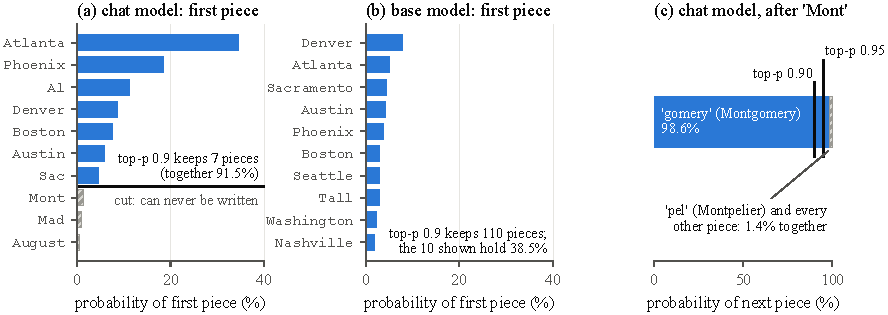
\includegraphics[width=\textwidth]{figures/fig1_mechanism.pdf}
  \caption{How a name becomes unreachable. Prompt: ``Name a capital city of a U.S. state.'' (a) The chat model's ten most likely first pieces. Top-p 0.9 keeps the 7 pieces above the line (91.5\% of the probability) and deletes the rest, so no capital starting with a deleted piece can be written. (b) The base model spreads its first step: its top piece has 7.8\% and top-p 0.9 keeps 110 pieces. (c) A name can also be cut later. After the shared piece `Mont', the chat model puts 98.6\% on `gomery' (Montgomery), so `pel' (Montpelier) is deleted even at top-p 0.95. Hatched: deleted pieces.}
  \label{fig:mechanism}
\end{figure*}

% Figure 2 (rbu_curves): generated by mb5.figures; inputs and hashes in sources.json
\begin{figure*}[t]
  \centering
  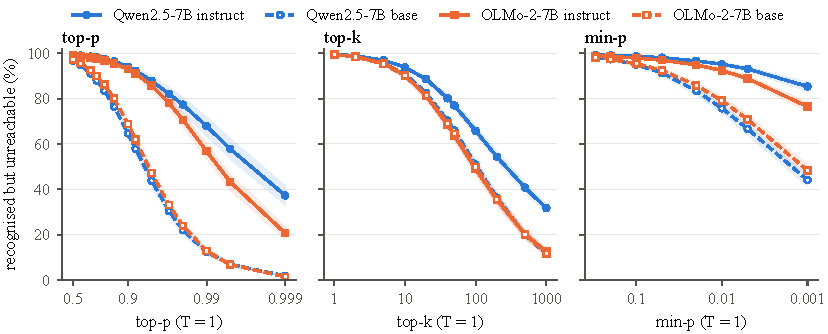
\includegraphics[width=\textwidth]{figures/fig2_rbu_curves.pdf}
  \caption{Share of recognised entities that are unreachable (RBU, exact verdict) as each truncation is loosened, full TailCat (277 categories), mean over three wordings with 95\% cluster-bootstrap bands. Left to right within each panel the truncation gets weaker. Solid, filled: post-trained (instruct) models; dashed, open: their base models. At top-p 0.9 the Qwen instruct model leaves 94.0\% unreachable against 64.7\% for its base model.}
  \label{fig:rbu_curves}
\end{figure*}

% Figure 3 (stages): generated by mb5.figures; inputs and hashes in sources.json
\begin{figure*}[t]
  \centering
  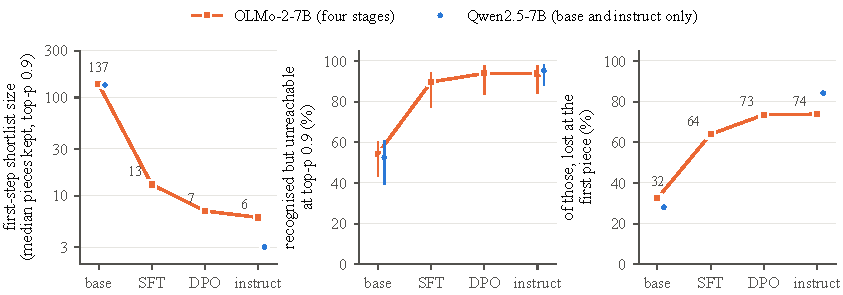
\includegraphics[width=\textwidth]{figures/fig3_stages.pdf}
  \caption{Where unreachability comes from: OLMo-2-7B after each post-training stage (pilot, 11 categories; SFT: supervised fine-tuning; DPO: preference tuning), with the Qwen2.5-7B base and instruct pair for comparison. SFT alone shrinks the first-step shortlist from 137 to 13 pieces. From base to instruct, the share of recognised entities that are unreachable at top-p 0.9 rises from 54.4\% to 93.8\%, and the share of those lost at the first piece from 32\% to 74\%. Bars: 95\% cluster-bootstrap intervals.}
  \label{fig:stages}
\end{figure*}

% Figure 4 (popularity): generated by mb5.figures; inputs and hashes in sources.json
\begin{figure}[t]
  \centering
  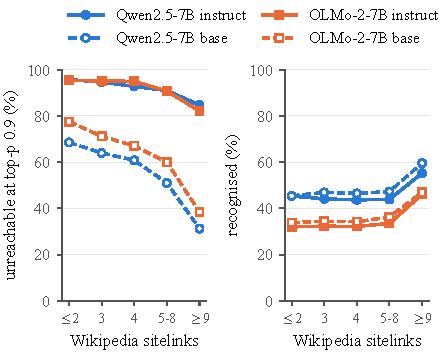
\includegraphics[width=\columnwidth]{figures/fig4_popularity.pdf}
  \caption{Who loses, on the full TailCat (33,437 members). Entities are binned by Wikipedia sitelinks (popularity quintiles; ties make the bins unequal). Left: share of recognised entities that are unreachable at top-p 0.9 (robust verdict). Right: share recognised. For the Qwen instruct model, unreachability falls from 95.8\% in the least linked bin to 84.7\% in the most linked bin.}
  \label{fig:popularity}
\end{figure}

% Figure 5 (estimators): generated by mb5.figures; inputs and hashes in sources.json
\begin{figure*}[t]
  \centering
  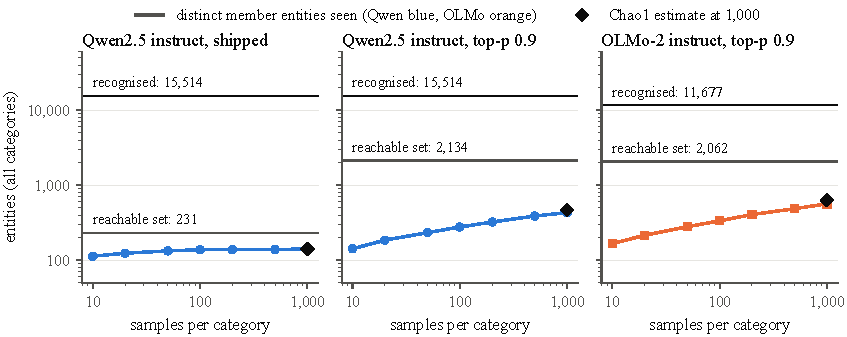
\includegraphics[width=\textwidth]{figures/fig5_estimators.pdf}
  \caption{Sample-based knowledge estimates see the reachable set, not what the model recognises (full TailCat, template 0, 1,000 samples per category). Curves: distinct member entities seen as samples grow; diamond: the Chao1 richness estimate from all samples; lines: the reachable set and the recognised set from the exact test. With the shipped sampler, Qwen yields 141 distinct members and Chao1 estimates 141, against 231 reachable and 15,514 recognised.}
  \label{fig:estimators}
\end{figure*}

% Figure 6 (frontier): generated by mb5.figures; inputs and hashes in sources.json
\begin{figure*}[t]
  \centering
  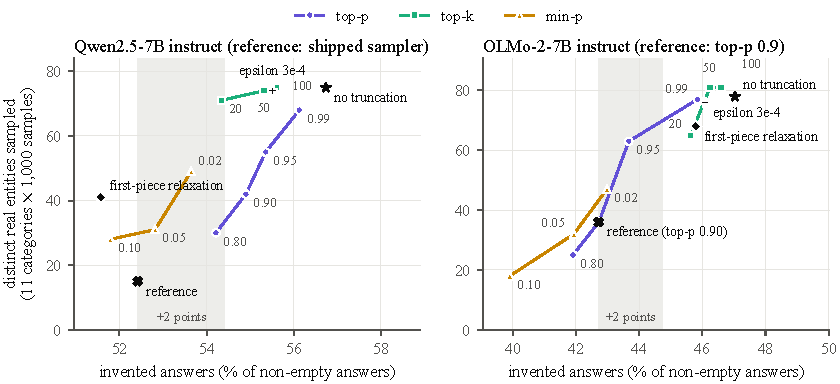
\includegraphics[width=\textwidth]{figures/fig6_frontier.pdf}
  \caption{The mitigation frontier (pilot, 11 categories, 1,000 samples per category and sampler). Each point is a sampler: distinct real member entities it produced against the share of answers that match no real member (``invented''; includes spelling variants and real names missing from Wikidata, see the hand audit). Lines join settings of one sampler family, labelled by their parameter. Shaded: within 2 points of the reference, the band gate G3 allowed. For Qwen, removing truncation raises distinct entities from 15 to 75 at 4.3 more points of invented answers.}
  \label{fig:frontier}
\end{figure*}
